\chapter{Colorings and symmetries}

In the previous chapters, we computed, how many proper colorings of Platonic and Archimedean solids exists using the notion of the chromatic polynomial. In that approach, we didn't take into account, that some colorings can be obtained from the other ones by simply rotating or reflecting the solid i.e. by applying some geometric transformation on it. When one coloring can be obtained from another one using some geometric transformation, then it makes good sense to regard these two colorings as identical. An analogy from chemistry is, that the properties of a molecule do not change, when we rotate it. Thus it is reasonable, to consider all its rotations as being the same molecule. 

In order to be able to say, which colorings should be considered identical, we need to define some kind of equivalence relation, that will group all the different transformations of same coloring together. In mathematics, we call this relation a \textit{transitivity relation} and its equivalence classes are typically referred to as its \textit{orbits}. The transitivity relation is defined on a set of objects, in our case the colorings, and a group that acts on these objects, the transformations.

Using the terminology above, our task boils down to counting the number of orbits of the transitivity relation, defined on colorings of our solid using the group of transformations of the solid.

To be able to use the transformations of the solids in our computations, we need a mathematical way of describing them. As we are working with graphs of the solids, we then also need to be able to describe these transformations as transformations on these graphs.


\section{Preliminaries}

It turns out, that transformations of the solid that we consider correspond exactly to automorphisms of the corresponding graph of the solid.

\begin{defn}[automorphism]
    Let $G=(V,E)$ be a graph. Then a function $f:V \rightarrow V$ is an \emph{automorphism} of $G$ if it is a bijection and for every $\{u,v\} \in E$ we have that $\{f(u),f(v)\} \in E$.
\end{defn}

For a graph $G$, we will denote the set of all automorphisms of $G$ by $\Aut(G)$.

\begin{defn}(group)
    A \emph{group} is a pair $\mathcal{G}=(G,\circ)$ where $G$ is a set, $\circ:G^2 \rightarrow G$ a binary operation s.t. the following hold:
    \begin{enumerate}
        \item $\forall x,y,z \in G : x \circ (y \circ z) = ( x \circ y ) \circ z$
        \item $\exists e \in G \ \forall x \in G :x \circ e = x = e \circ x$
        \item $ \forall x \in G \ \exists y \in G : x \circ y = e = y \circ x$
    \end{enumerate}
\end{defn}

An important observation is, that for a graph $G$, the set of all automorphisms $\Aut(G)$ together with the function composition operation forms a group. 

Before we define can define the transitivity relation, we also need to properly define the set of elements on which this relation will be defined:

\begin{defn}[colorings with up to n colors]
    For a graph $G$, positive integer $n$ and a family of colorings $C$, we define the set $C_n \subseteq C$ the set of all proper colorings of $G$ by at most $n$ colors.
\end{defn}

The definition above restricts the colorings we will be working with to finite sets only. With the notion of automorphism and colorings in hand, we can define the transitivity relation for the colorings.

\begin{defn}(transitivity relation)
        Let $G=(V,E)$ be a graph and $n\in \mathbb{N}$. Let $c_1,c_2 \in C_n$. We define $c_1 \sim c_2$ whenever exists an automorphism $\pi \in \Aut(G) : \forall v \in V : c_1(v)=c_2(\pi(v))$.
\end{defn}

Less formally, two colorings are related, when we can find an automorphism that maps vertices of any color in the first coloring, to vertices of the same color in the second coloring. 

We can observe that for any coloring $c$ of $G$, we have $c \sim c$ by simply taking the identity automorphism $id \in \Aut(G)$. So the transitivity relation is \textit{reflexive}. It is also \textit{symmetric} by using the fact, that if $c_1 \sim c_2$ by existence of automorphism $\pi$, then we can use $\pi^{-1}$ to show that $c_2 \sim c_1$ as well. Lastly, we can also show that the relation $\sim$ is \textit{transitive}. This comes from the fact, that composing two automorphisms $\pi$ and $\psi$ yields an automorphism. So in fact, the transitivity relation defined above is an eqivalence relation.

\begin{defn}(orbit)
    For $n \in \mathbb{N}$ and a coloring $c \in C_n$ of some graph $G$ we will call the eqivalence class $[c]_{\sim}$ an \emph{orbit} of $c$ and denote it by $\Orb(c)$.
\end{defn}

\begin{defn}(set of all orbits)
    For $n \in \mathbb{N}$ and a set $C_n$ of proper colorings of graph $G$, we denote $C_n/_\sim$ the set of all eqivalence classes of the transitivity relation $\sim$ on $C_n$.
\end{defn}

Here is a good place to point out, that it is exactly our objective, to calculate the size of this set, $\abs{C_n/_\sim}$.

\begin{defn}(stabilizer)
    For $n \in \mathbb{N}$ and a coloring $c \in C_n$ of $G=(V,E)$, we will call the set $\Stab(c) = \{ \pi \in \Aut(G) \ | \ \forall v \in V : c(\pi(v)) = c(v) \}$ a \emph{stabilizer} of $c$. 
\end{defn}

Again, to say more coloquially, the stabilizer is the set of all automorphisms that when applied to a coloring will result in exactly the same coloring. What we mean by same colorings is, that all the vertices get the same color under both colorings.

\section{Calculating the number of orbits}

Now it can be shown using the Lagrange's theorem that $\abs{\Stab(c)} \cdot \abs{\Orb(c)} = \abs{\Aut(G)}$ which is the key fact that allows us to be able to compute the number of equivalence classes of the transitivity relation. Mathematically formulated, it allows us to derive the following equation:

\begin{equation}\label{eqn:orbits-by-stab}
    \sum_{c\in C_n}\abs{\Stab(c)} = \abs{\Aut(G)} \cdot \abs{C_n/_\sim} 
\end{equation}


Usually, this formula is not suitable for practical calculations because the size of set $C_n$ can be quite large. In most cases, the set $\Aut(G)$ is much smaller and thus it is more reasonable, to sum over its elements instead. 

For example, consider the graph of cube $G_{cube}$. Taking for $C_4$ the set of all proper colorings of $G_{cube}$ by at most $4$ colors, we get $\abs{C_4} = 2652$. This value can be obtained by plugging number $4$ to the chromatic polynomial of $G_{cube}$. On the other hand, by consulting table \ref{tab:plat-automorphisms} below, we have $\abs{\Aut(G_{cube})} = 48$ which is more than hundred times smaller number.

Before stating another important observation, we will need a following definition:

\begin{defn}[fixpoint]
    For a graph $G$, $n \in \mathbb{N}$, a set of its proper colorings $C_n$ and automorphism $\pi \in \Aut(G)$ we denote $\Fix(\pi)= \{ c \in C \ | \ \forall v \in V : c(\pi(v)) = c(v) \}$
\end{defn}

To get a formula which computes the same number but using a sum over the set $\Aut(G)$ instead, we use the following observation: The sum $\sum_{c \in C_n} \abs{\Stab(c)}$ computes the number of ordered pairs $(c,\pi)$ s.t. $\forall v \in V : c(\pi(v)) = c(v)$. Using the definition of fixpoint, we can calculate this number also using the sum $\sum_{\pi \in \Aut(G)} \abs{\Fix(\pi)}$ which yields the following important identity:
\begin{equation}\label{eqn:two-way-counting}
    \sum_{\pi \in \Aut(G)} \abs{\Fix(\pi)} = \sum_{c \in C_n}\abs{\Stab(c)}    
\end{equation}

By combining equations \ref{eqn:orbits-by-stab} and \ref{eqn:two-way-counting}, we get the following result which is a direct application of the famous \textit{Burnside's lemma} on our particular setting:

\begin{thm}[application of Burnside's lemma] \label{thm:burnside}
    For a graph $G$, $n \in \mathbb{N}$ and a set of its proper colorings $C_n$, we have:
    $$\abs{C_n/_\sim} = \frac{1}{\abs{\Aut(G)}}\cdot \sum_{\pi \in \Aut(G)}\abs{\Fix(\pi)}$$
\end{thm}

\section{Orbital chromatic polynomial}

We introduce a notion very similar to the one of the chromatic polynomial of a graph. Additionally, we take into account symmetries.

\begin{defn}[orbital chromatic polynomial]
    For a graph $G$ and a family of its proper coloring $C$ we define the \emph{orbital chromatic polynomial} $OP(G,x)$ as a polynomial s.t. $\forall k \in \mathbb{N} : OP(G,k)$ is equal to $\abs{C_k/_\sim}$
\end{defn}

The notion of orbital chromatic polynomial was first introduced by Cameron and Kayibi \cite{caka2007} in 2007 and was defined in more general terms for any subgroup of automorphisms $A \leqslant  \Aut(G)$. In the following section, some of the definitions are adaptations of similar definitions also from \cite{caka2007}. The Theorem \ref{thm:count-orb-chrompoly} is equivalent to how the orbital chromatic polynomial was defined in \cite{caka2007}. In this thesis, we provide a more detailed proof of the method outlined in \cite{caka2007}. 

For a graph $G$ the orbital chromatic polynomial $OP(G,x)$ can be expressed in terms of the usual chromatic polynomial. But in order to do so, it is helpful to define a special kind of graph. We define it in terms of a given automorphism $a$ and call it the \textit{fixation graph}. Any coloring $c' \in C'_n$ of the fixation graph corresponds exactly to one coloring $c \in C_n$ of the original graph $G$ that is fixed by the automorphism $a$.

\begin{defn}[cycles of permutation]
    Given a graph $G=(V,E)$ and an automorphism $\pi \in \Aut(G)$ we denote the set of cycles of $\pi$ by $\Cycles(\pi)$. By a cycle $O \in \Cycles(\pi)$, we mean the set of vertices of $G$ on the cycle $O$.
\end{defn}

\begin{defn}[vertex set identification]
    For a graph $G=(V,E)$ a subset of vertices $S \subseteq V$ we define the \emph{identification of vertex set $S$} into a new vertex $w \notin V$ as the operation that results in a graph $G_{\star,S}=(V',E')$ defined as follows:
    \begin{enumerate}
        \item $V' := (V \setminus S) \cup \{w\}$
        \item $E' := \left( \binom{V'}{2} \cap E\right) \cup \{ \{w,x\} \ | \ (\exists x \in V \setminus S)(\exists s \in S): \{x,s\} \in E\}$
    \end{enumerate}
\end{defn}

Given a graph $G=(V,E)$ and a sequence of disjoints subsets $S_1, \ldots , S_n \subseteq V$, we denote $G_{\star,S_1,\ldots,S_n}$ the graph resulting from successive application of vertex set identification operation on the sets $S_1$ up to $S_n$ and graph $G$.

\begin{defn}[independent set]
    For a graph $G=(V,E)$ and a subset of vertices $S \subseteq V$, we say that $S$ is \emph{independent} if $\forall x,y \in S : \{x,y\} \notin E$.
\end{defn}

In the following definition, we extend the definition of an undirected graph to allow also \textit{loops}. By a loop $l \in \binom{E}{1}$, we mean an edge with both endpoints being an identical vertex. For any graph $G$ containing a loop $l$, we set the chromatic polynomial $P(G,x) = 0$.

\begin{defn}[fixation graph]
    Given a graph $G$ and automorphism $\pi \in \Aut(G)$. For $n = \abs{\Cycles(\pi)}$ let $O_1, \ldots ,O_n \subseteq \Cycles(\pi)$ be the sequence of cycles of $\pi$ in an arbitrary order. We define the \emph{fixation graph} $G /_{\pi}$ as $G_{\star,O_1, \ldots , O_n}$ s.t. additionally, we add a loop at every new vertex $w_i$ if $O_i$ was not an independent set.
\end{defn}

Now we are ready to state the following theorem:

\begin{thm}[computation of orbital chromatic polynomial] \label{thm:count-orb-chrompoly}
    Let $G$ be a graph, then the following formula holds:
    \begin{equation} \label{eqn:oribtal-chrompoly}
        OP(G,x) = \frac{1}{\abs{\Aut(G)}} \cdot \sum_{\pi \in \Aut(G)}P(G/_\pi,x)
    \end{equation}
\end{thm}

\begin{proof}
    We show that for any positive integer $n$ we have: $$OP(G,n) = \frac{1}{\abs{\Aut(G)}} \cdot \sum_{\pi \in \Aut(G)}P(G/_\pi,n)$$

    Let $G=(V,E)$ be a graph and $n \in \mathbb{N}$. By definition of orbital chromatic polynomial we have $OP(G,n) = \abs{C_n /_{\sim}}$. So by the Burnside's orbit counting lemma \ref{thm:burnside} we have:
    $$OP(G,n) = \frac{1}{\abs{\Aut(G)}} \cdot \sum_{\pi \in \Aut(G)} \abs{\Fix(\pi)}$$

    In order to prove the equation above, it is enough to show that $\forall \pi \in \Aut(G) : P(G/_{\pi},n) = \abs{\Fix(\pi)}$. Formally, we need to find a one-to-one correspondence between any coloring $c \in \Fix(\pi)$ and a coloring $c' \in C'_n$ where $C'_n$ is the set of all colorings of $G /_\pi = (V',E')$ using at most $n$ colors. It will be helpful, for $k = \abs{\Cycles(\pi)}$, to denote $w_1, \ldots , w_k$ the new vertices corresponding to the cycles $O_1, \ldots ,O_k \in \Cycles(\pi)$ that were identified in $G$ to get the resulting graph $G/_\pi$.
    
    Let $c \in \Fix(\pi)$ be a coloring of $G$ that is fixed by $\pi$. Because $c$ is fixed by $\pi$, then by definition, it must hold that $\forall v \in V : c(\pi(v)) = c(v)$. By this condition, for a given cycle $O_i \in \Cycles(\pi)$, we have that $\forall u,v \in O_i : c(u) = c(v) = b_i$ for some color $b_i$ i.e. all vertices on a cycle must have the same color $b_i$. Note that we allow for $i \neq j$ to have $b_i = b_j$. Now we map the proper coloring $c \in C_n$ to a coloring $c' \in C'_n$ defined s.t. $\forall i \in \{1, \ldots ,k\} : c'(w_i) = b_i$. This results in a proper coloring since if for any $i \neq j$ we have $\{w_i,w_j\} \in E'$ then there must exist vertices $u \in O_i$ and $v \in O_j$ s.t. $\{u,v\} \in E$ by the definition of vertex set identification operation. Thus we have $b_i \neq b_j$. So we have $c' \in C'_n$. 
    
    Now suppose that we have $c_1,c_2 \in C_n$ s.t. $c_1 \neq c_2$ then the images under this mapping $c'_1,c'_2 \in C'_n$ are different so the mapping is injective.

    For surjectivity, suppose we have a proper coloring $c' \in C'_n$ of graph $G/_\pi$. Then the preimage of $c'$ is the following coloring which we denote by $c \in C_n$: $(\forall O_i \in \Cycles(\pi))( \forall v \in O_i) : c(v) = c'(w_i)$. It is not hard to see, by the definition of the vertex set identification operation, that the coloring $c$ is a proper coloring of $G$. Note that we also have that $c \in \Fix(\pi)$ because we assigned all vertices on each cycle the same color.

    So we have that $\forall \pi \in \Aut(G) : P(G/_{\pi},n) = \abs{\Fix(\pi)}$. 

    \vspace{5pt}
    \todo{TODO: Now we have to show that if for all $n \in \mathbb{N}$ the polynomials have equal value, then they are indeed equal. This would be true if we could somehow limit the degree of OP (the orbital chromatic polynomial)}
     
\end{proof}

\section{Calculating orbital chromatic polynomials}

Theorem \ref{thm:count-orb-chrompoly} can be used to derive a following algorithm:

\begin{algorithm}[H]
    \caption{Algorithm based on Theorem \ref{thm:count-orb-chrompoly} for computing the orbital chromatic polynomial $OP(G,x)$ of a given graph $G$} 
    \begin{algorithmic}[1]
        \Function{OrbitalChromaticPoly}{$x$}
            \State $p \gets 0$      
            \For{$\pi \in \Aut(G)$}
                \State $H \gets G$
                \For{$O \in \Cycles(\pi)$}
                    \If{$O$ not independent set}
                        \State Continue with next permutation at step $3$
                    \EndIf
                    \State $H \gets H_{\star,O}$
                \EndFor
                \State $p \gets p + P(H,x)$
            \EndFor   
            \State \Return $p$
        \EndFunction
    \end{algorithmic}
    \label{alg:orb-chrompoly}
\end{algorithm}

An implementation of the algorithm \ref{alg:orb-chrompoly} above is provided in the appendix. This implementation was used to calculate the polynomials that can be seen in table \ref{tab:selected-orbital-chrom-polys} below.

\renewcommand{\arraystretch}{2.0}
\begin{table}[H]
\centering
\begin{tabular}{l@{\hspace{1.5cm}}p{0.7\linewidth}}
\toprule
\textbf{Solid} & \textbf{Orbital chromatic polynomial} \\
\midrule
tetrahedron & $\frac{1}{24}x^{4} - \frac{1}{4}x^{3} + \frac{11}{24}x^{2} - \frac{1}{4}x$ \\
octahedron & $\frac{1}{48}x^{6} - \frac{3}{16}x^{5} + \frac{37}{48}x^{4} - \frac{79}{48}x^{3} + \frac{41}{24}x^{2} - \frac{2}{3}x$ \\
cube & $\frac{1}{48}x^{8} - \frac{1}{4}x^{7} + \frac{3}{2}x^{6} - \frac{16}{3}x^{5} + \frac{193}{16}x^{4} - \frac{203}{12}x^{3} + \frac{161}{12}x^{2} - \frac{9}{2}x$ \\
\bottomrule
\end{tabular}
\caption{Orbital chromatic polynomial of selected solids.}
\label{tab:selected-orbital-chrom-polys}
\end{table}
\renewcommand{\arraystretch}{1.0}

\subsection{Demonstrative example on a graph of the octahedron}

The difference between chromatic and orbital chromatic polynomials can be demonstrated on a graph of the octahedron $K_{3 \times 2}$. As can be seen in table \ref{tab:selected-chrom-polys} we have that: $$P(K_{3 \times 2},x) = x^{6} - 12x^{5} + 58x^{4} - 137x^{3} + 154x^{2} - 64x$$ whereas by \ref{tab:selected-orbital-chrom-polys} 
 we have: $$OP(K_{3 \times 2},x) = \frac{1}{48}x^{6} - \frac{3}{16}x^{5} + \frac{37}{48}x^{4} - \frac{79}{48}x^{3} + \frac{41}{24}x^{2} - \frac{2}{3}x$$.

Plugging in $3$ for $x$, we get the number of vertex colorings of the octahedron using at most $3$ colors. We get $P(K_{3 \times 2},3) = 6$. All these colorings can be enumerated using \textit{SageMath} \cite{sagemath} and its \verb|all_graph_colorings| function. On the figure below, we can see all of these $6$ colorings:

\begin{figure}[H]
    \centering
    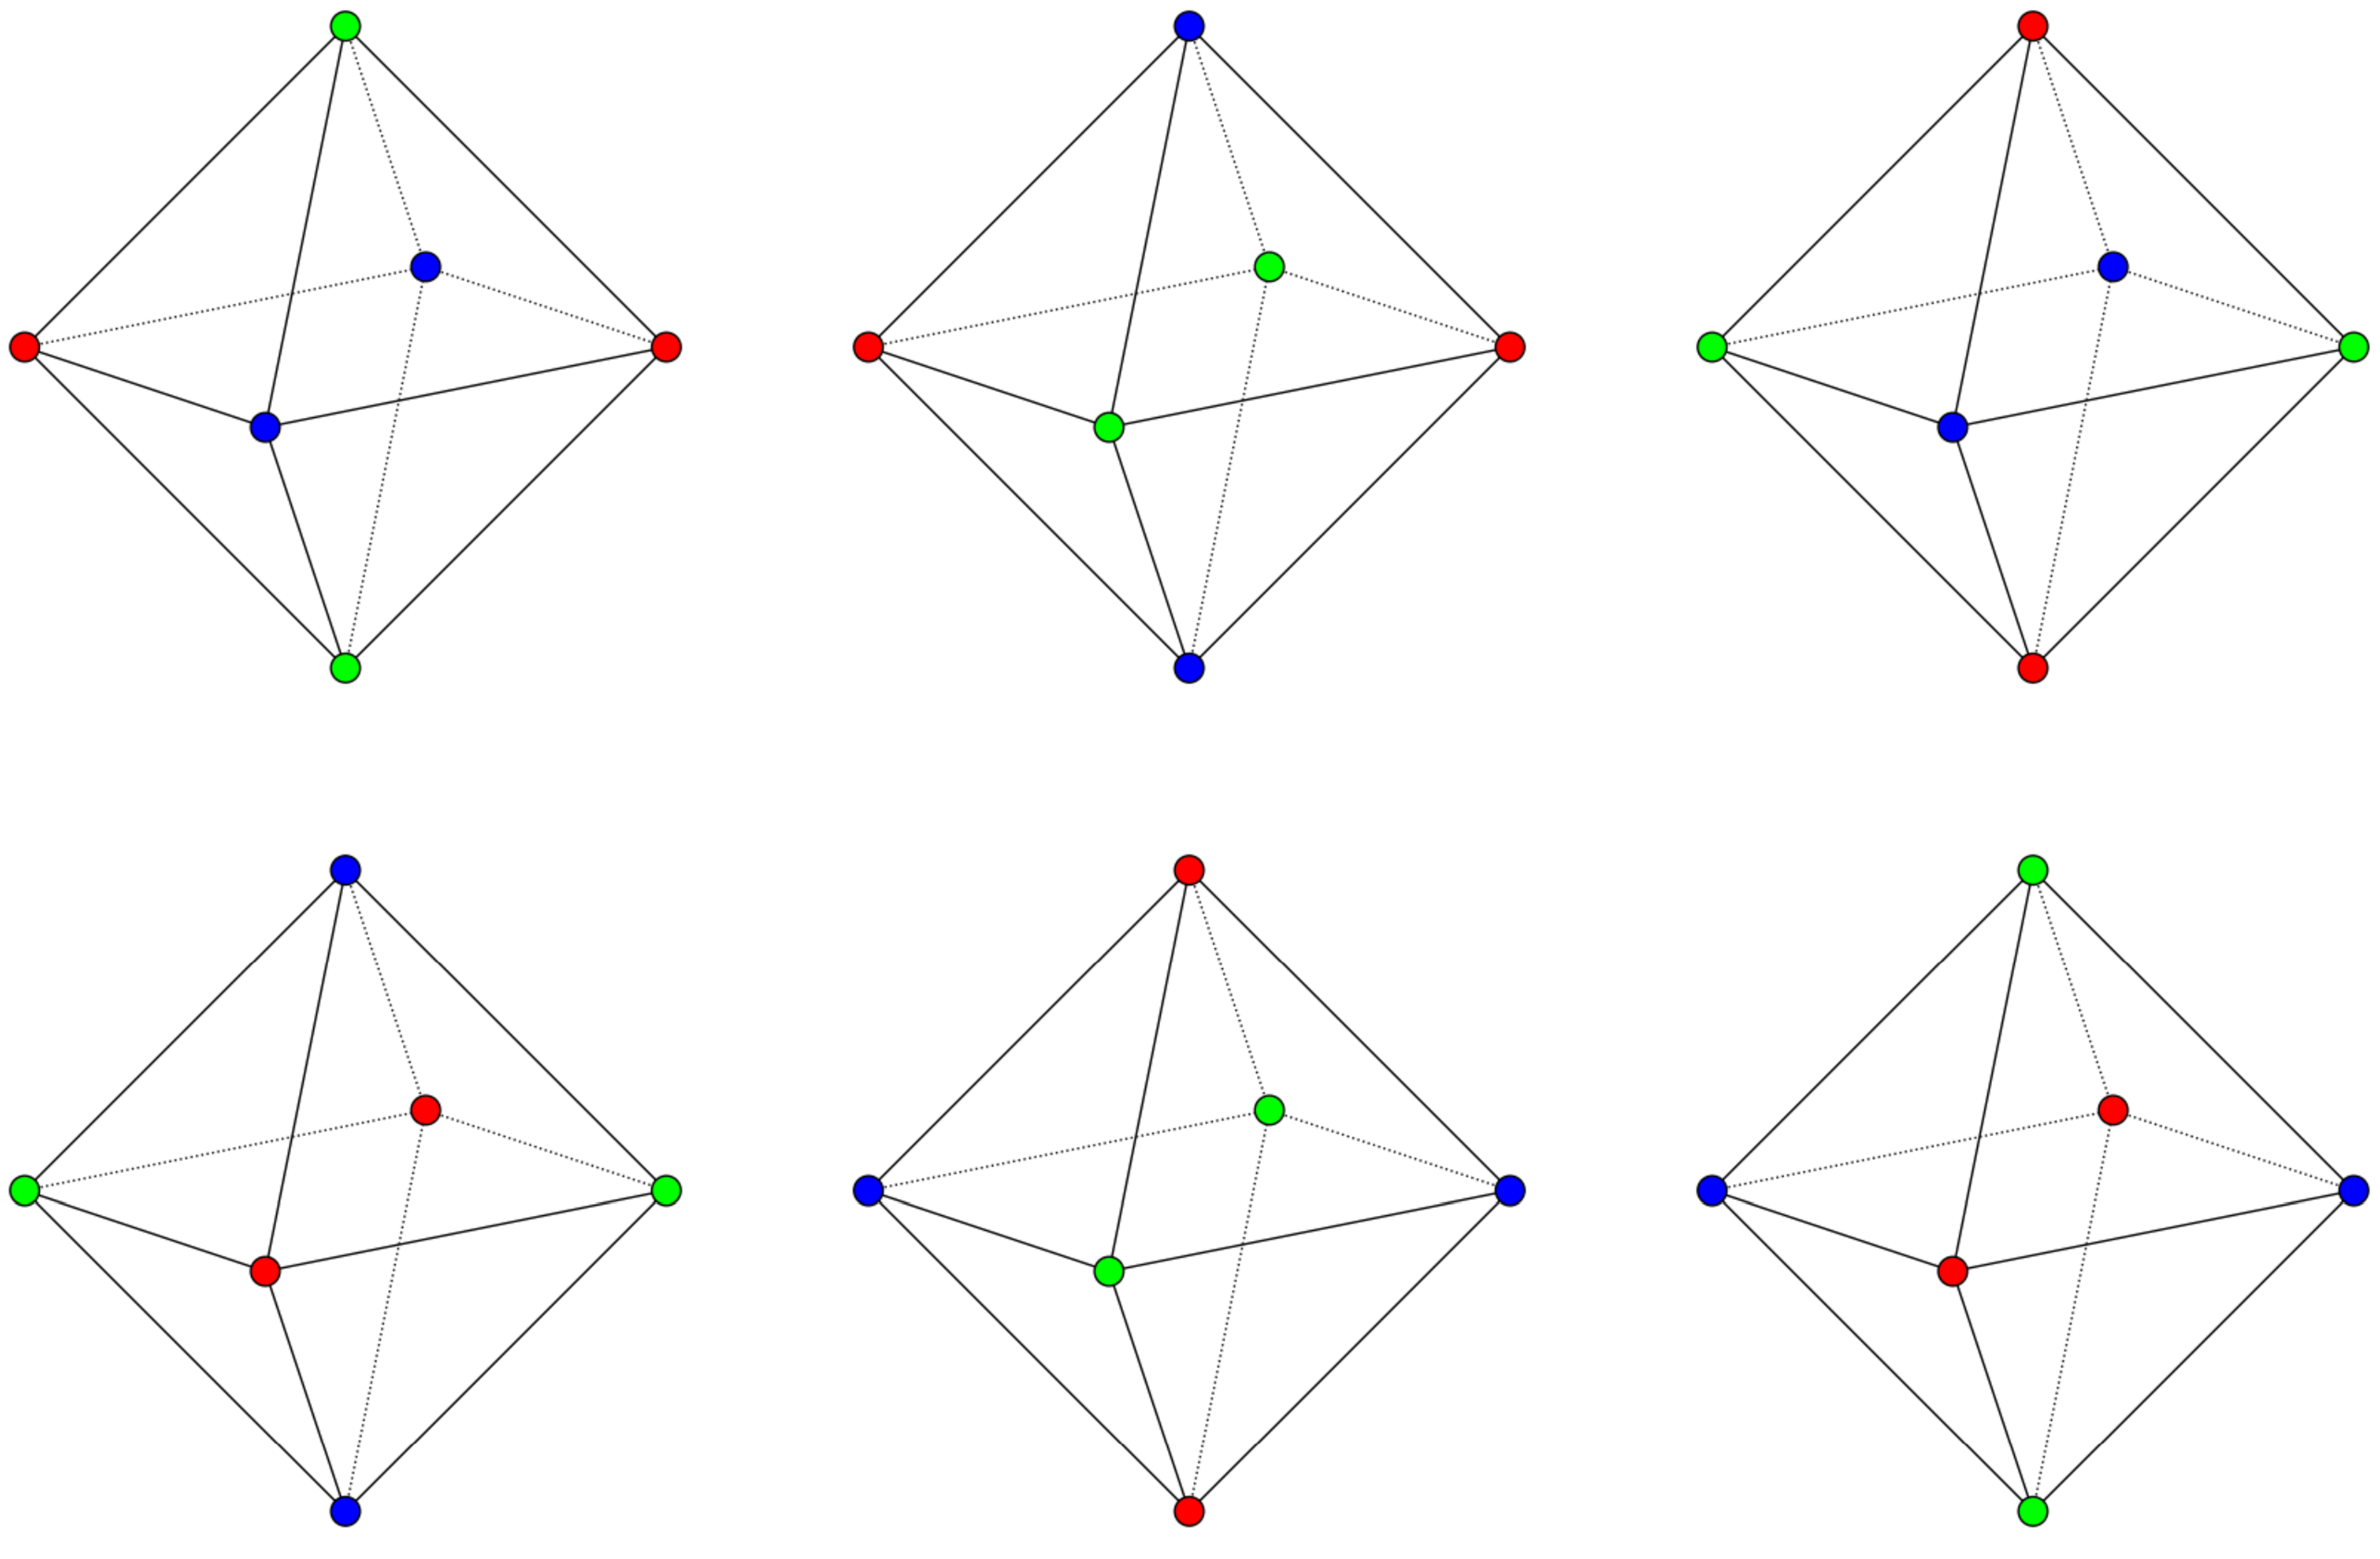
\includegraphics[width=1\textwidth]{../Resources/Figs/octahedron_3-clrings.pdf}
    \caption{All 3 colorings of octahedral graph}
    \label{fig:octahedron-3-clrings}
\end{figure}

Now, an important observation is, that all of these $6$ colorings are equivalent when considered up to automorphisms. Indeed we can compute that $OP(K_{3 \times 2},3) = 1$.

\todo[JF]{Hezká ukázka, ale ne moc překvapivá. Co třeba kdybyste ještě přidal 3-obarvení krychle, nevyjde to zajímavěji? Nebo 3-obarvení dvanáctistěnu. 

Kolik takových vlastně je? Možná by mělo smysl je dát do tabulky.
Např pro krychli počet všech / počet různých pro 2 až 8 barev.}

\begin{highlight}

\section{Comparison of evaluations of both types of polynomials}

It is interesting to compare the difference between chromatic polynomial and orbital chromatic polynomial for all the solids by looking at the values of the polynomials at certain points. This can be seen in table \ref{tab:platonic-polys-evals} below.

\begin{table}[H]
\centering
\begin{tabular}{l@{\hspace{0.5cm}}ccccccc}
\toprule
\textbf{Platonic solid} & \textbf{2} & \textbf{3} & \textbf{4} & \textbf{5} & \textbf{6} & \textbf{7} & \textbf{8} \\
\midrule
tetrahedron & $0$ & $0$ & $24$ & $120$ & $360$ & $840$ & $1680$ \\
 & $0$ & $0$ & $1$ & $5$ & $15$ & $35$ & $70$ \\
\specialrule{0.2pt}{0.65ex}{0.65ex}
octahedron & $0$ & $6$ & $96$ & $780$ & $4080$ & $15330$ & $45696$ \\
 & $0$ & $1$ & $10$ & $55$ & $215$ & $665$ & $1736$ \\
\specialrule{0.2pt}{0.65ex}{0.65ex}
cube & $2$ & $114$ & $2652$ & $29660$ & $198030$ & $932862$ & $3440024$ \\
 & $1$ & $15$ & $154$ & $1115$ & $5955$ & $24836$ & $85260$ \\
\specialrule{0.2pt}{0.65ex}{0.65ex}
icosahedron & $0$ & $0$ & $240$ & $80400$ & $4012560$ & $\approx 10^{7}$ & $\approx 10^{8}$ \\
 & $0$ & $0$ & $2$ & $670$ & $33444$ & $640444$ & $6878900$ \\
\specialrule{0.2pt}{0.65ex}{0.65ex}
dodecahedron & $0$ & $7200$ & $\approx 10^{8}$ & $\approx 10^{11}$ & $\approx 10^{13}$ & $\approx 10^{14}$ & $\approx 10^{16}$ \\
 & $0$ & $75$ & $1404848$ & $\approx 10^{8}$ & $\approx 10^{11}$ & $\approx 10^{12}$ & $\approx 10^{14}$ \\
\bottomrule
\end{tabular}
\caption{Evaluated chromatic polynomial and orbital chromatic polynomial for platonic solids at points 2 to 8. For each solid, the top row contains the chromatic polynomial, the bottom row contains the orbital chromatic polynoial.}
\label{tab:platonic-polys-evals}
\end{table}

It is important to note, that in table \ref{tab:platonic-polys-evals} above, in column $n$, the entry does not correspond to the amount of colorings with exactly $n$ colors but with at most $n$ colors. This means, that colorings that used only a proper subset of the $n$ available colors are counted as well.

\section{Number of colorings using exactly n colors}

Let us denote $!P(G,n)$ the amount of colorings of graph $G$ using \emph{exactly} $n$ colors. This number can be calculated using a recursive formula with a base case being $!P(G,\chi(G))=P(G,\chi(G))$. The recursive formula is as follows:
\begin{equation}\label{eqn:exactly-n-colors}
!P(G,n) = P(G,n) - \sum_{i=\chi(G)}^{n-1}\binom{n}{i}!P(G,i)    
\end{equation}

\begin{proof}
    For the base case, it is trivial to show that $!P(G,\chi(G))=P(G,\chi(G))$ since there exist no colorings that use less than $\chi(G)$ colors.
    
    For the recursive case, let $n>\chi(G)$ be the number for which we want to calculate $!P(G,n)$. We proceed by taking the value $P(G,n)$ and noticing, that this value also calculates colorings using $n-1$, $n-2$, \ldots \ , $\chi(G)$ colors which we want to exclude. For $i \in \{\chi(G),\ldots,n-1\}$ how many colorings using $i$ colors have we calculated? A naive approach would be to simply subtract the value $!P(G,i)$. The problem with this approach is, that when we are allowed to use $n$ colors and have to use exactly $i$ of them, we can choose the set of $i$ colors to use in $\binom{n}{i}$ ways. Note that indeed all of the $\binom{n}{i}$ colorings use at most $n$ colors and are pairwise different. Using this observation, we can see that the correct amount to subtract is $\binom{n}{i}!P(G,i)$ for each $i$.
\end{proof}

Note that formula \ref{eqn:exactly-n-colors} above holds also for the orbital chromatic polynomial $OP(G,x)$ and corresponding values $!OP(G,n)$. Using these formulas, we can then simplify table \ref{tab:platonic-polys-evals} above to get a following table:

\begin{table}[H]
\centering
\begin{tabular}{l@{\hspace{0.5cm}}ccccccc}
\toprule
\textbf{Platonic solid} & \textbf{2} & \textbf{3} & \textbf{4} & \textbf{5} & \textbf{6} & \textbf{7} & \textbf{8} \\
\midrule
tetrahedron & $0$ & $0$ & $24$ & $0$ & $0$ & $0$ & $0$ \\
 & $0$ & $0$ & $1$ & $0$ & $0$ & $0$ & $0$ \\
\specialrule{0.2pt}{0.65ex}{0.65ex}
octahedron & $0$ & $6$ & $72$ & $360$ & $720$ & $0$ & $0$ \\
 & $0$ & $1$ & $6$ & $15$ & $15$ & $0$ & $0$ \\
\specialrule{0.2pt}{0.65ex}{0.65ex}
cube & $2$ & $108$ & $2208$ & $17520$ & $57600$ & $80640$ & $40320$ \\
 & $1$ & $12$ & $100$ & $485$ & $1290$ & $1680$ & $840$ \\
\specialrule{0.2pt}{0.65ex}{0.65ex}
icosahedron & $0$ & $0$ & $240$ & $79200$ & $3533760$ & $\approx 10^{7}$ & $\approx 10^{8}$ \\
 & $0$ & $0$ & $2$ & $660$ & $29454$ & $420336$ & $2654400$ \\
\specialrule{0.2pt}{0.65ex}{0.65ex}
dodecahedron & $0$ & $7200$ & $\approx 10^{8}$ & $\approx 10^{11}$ & $\approx 10^{13}$ & $\approx 10^{14}$ & $\approx 10^{16}$ \\
 & $0$ & $75$ & $1404548$ & $\approx 10^{8}$ & $\approx 10^{11}$ & $\approx 10^{12}$ & $\approx 10^{14}$ \\
\bottomrule
\end{tabular}
\caption{Numbers of colorings using exactly 2 to 8 colors. For each solid, the top row contains the value when counting also symmetric colorings as different. The bottom row takes two colorings as different only if they cannot be identified using some automorphism.}
\label{tab:platonic-exactly-n-clrs}
\end{table}

\vspace{5pt}
\todo{TODO: Add visual example of 3-colorings of cube up to automorphisms.}

\section{Counting partitionings into independent sets}

Important thing to note about results of table \ref{tab:platonic-exactly-n-clrs} above is the fact, that we count two colorings $c_1$ and $c_2$ as different also in the case, when $c_1$ can be obtained as a permutation of colors of $c_2$. This is something we would like to avoid if we are interested in the structure of the coloring only and the value of the colors bear no special meaning for us. 

In order to achieve the above, we have to view the coloring as a partitioning into independent sets, where the sets have no labels. Now, let us count the amount of partitions where we exclude same partitionings that only differ by their colors. For each coloring using exactly $k$ colors, we have exactly $k$ partitions. Imagine the colors as $k$ labels we would like to use to label the $k$ partitions, then there is exactly $k!$ ways to label them. 

\end{highlight}